\section{Krabice}
Vzhledem k tomu že dveře trezoru (o kterých je tato práce) jsou schopny se zamčít do čehokoli se správným tvarem otvoru, je možné velice jednoduše navrhnout libovolnou krabici které by mé 
dveře sloužili jako zamykatelné víko. 

Aby trezor mohl sloužit (alespoň teoreticky) jako opravdoví trezor, a ne jen jako hračka, navrhl jsem i bezpečnostní stránku do zdi. Vzhledem k velikosti dveří by totiž ani nedobytná schránka 
nebyla bezpečná jelikož by se dala jednoduše přenést celá. Proto jsem zvolil schránku umístěnou ve zdi. 

\begin{figure}[htbp]
    \centering
    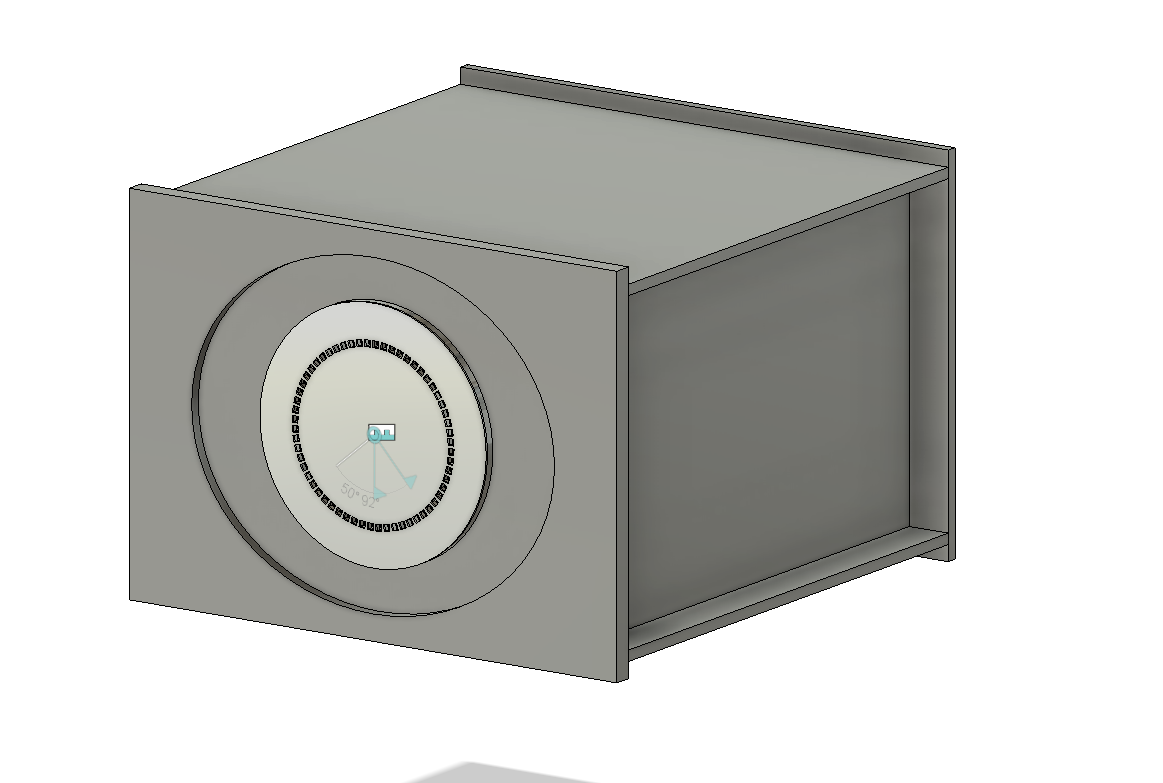
\includegraphics[width=240pt]{kapitoly/obrazky/E4/bedna/bedna.png}
    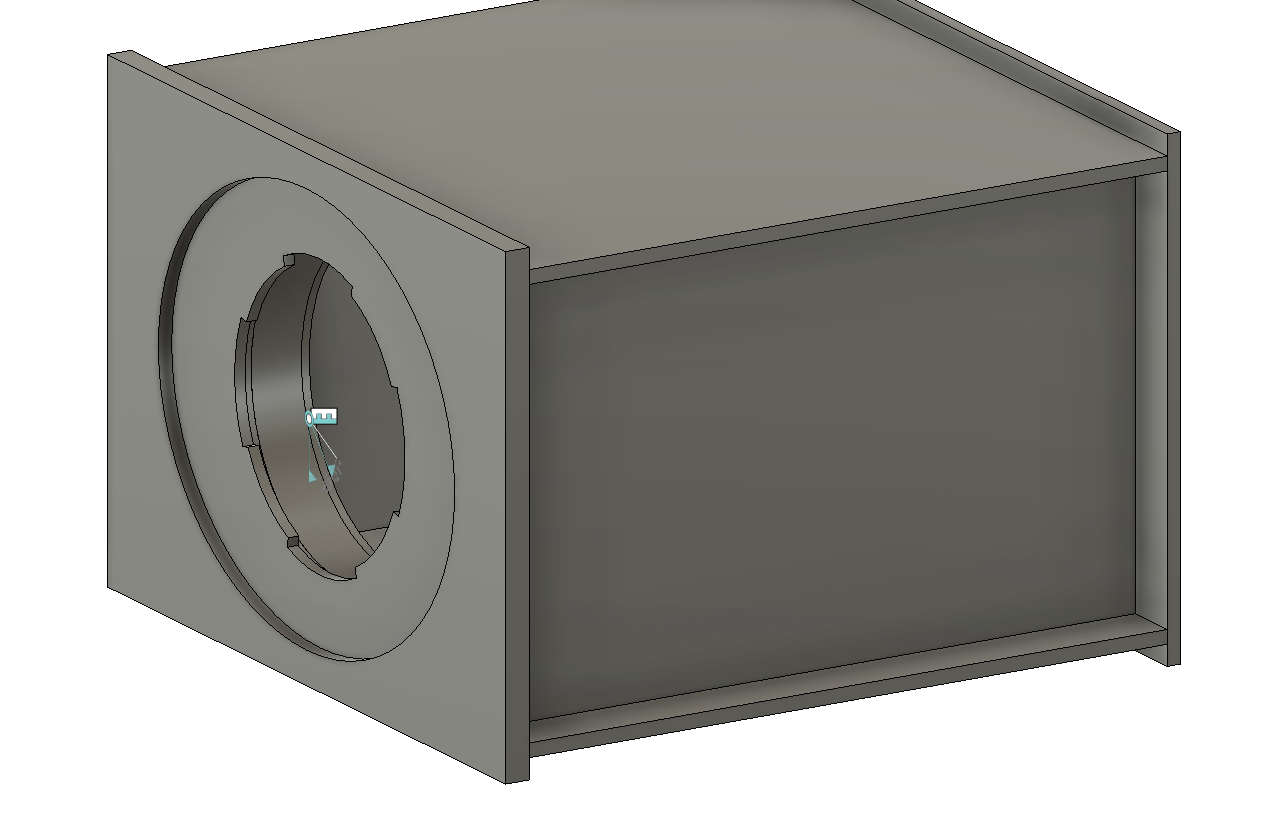
\includegraphics[width=240pt]{kapitoly/obrazky/E4/bedna/jen-bedna.png}
    \caption{Bedna}
    \label{fig:E4-bedna}
\end{figure}

Tato krabice by měla mít odolnou přední stěnu, ty ostatní by pak měli zajišťovat jen pevné uchycení ve stěne.